\documentclass{article}
\usepackage[brazil]{babel}
\usepackage[utf8]{inputenc}
\usepackage{url}
\usepackage{multicol}
\usepackage[bottom=2cm,top=2cm,left=2cm,right=2cm]{geometry}
\usepackage{graphicx}
\usepackage{float}
\usepackage{caption}
\usepackage[dvipsnames]{xcolor}
%\usepackage{subcaption}

\usepackage{setspace}
\usepackage{indentfirst}
\usepackage{mathtools}
\usepackage{amsmath}
\usepackage{subfigure}

\title{Fundamentos de Astronomia\\
    \large \texttt{[AGA0215]}\\
    \large Prof Auguto Damineli\\
    \large Prof Eduardo Cypriano}

\author{Julia Leite}

\begin{document}
    
\maketitle

\tableofcontents

\newpage

\section{Astronomia e humanidade}

\subsection{Origem}

Texto mais antigo sobre astronomia encontrado na mesopotâmia (atual
Iraque) tem observações sobre o planeta Vênus, datado de 1600 a.C.

Existem gravuras mais antigas, mas que não podem ser traduzidos como 
dados, originados da China, de 2700 a.C., da Irlanda (de 3400 a.C.),
França (17 000 a.C.), entre outros....

Até animais se guiam pelos padrões dos astros, como as aves migratórias
e as plantas (fototropismo)

Antiguidade havia necessidade de entender e gerenciar os ciclos de 
tempo (estações) para saber quando plantar, estocar, etc.

Primeiro, usando a Lua para marcar tempo e estações. Só que o ciclo 
tem 29 dias e meio, então a cada 2 anos o calendário estava quase um mês
atrasado.

Depois, o Sol passou a ser usado como referência, por exemplo, quando 
ele nascia e se punha perto da estrela Aldebaran as vacas engravidaram
e a constelação (estelas perto) foi chamada de touro, simbolizando a 
primavera. Quando Regulus nascia antes do sol, começava o verão e 
foi criada a constelação de Leão. Fomalhaut indicava o outovo e Antares, o inverno. 

Essas 4 estrelas marcavam o deslocamento do sol ao longo do ano e a 
tragetória foi chamada de Zodíaco (caminho dos animais)

No Egito, as estrelas eram usadas no lugar da Lua para determinar a 
duração do ano com maior precisão, o que permitiu a formação de cidades,
excedentes na agricultura, tempo de ócio, ... 

A observação do céu também remonta a motivos religiosos, há registros 
em povos extintos da Austrália, nos guaranis, nos mesopotâmios, entre 
outros. Isso se reflete na origem da serpente como símbolo da medicina
(serpente Tiamat que traz a ideia de fazer uma viagem ritual às origens
do universo, quando não existia doença), reveillon (festa da primavera),
Natal, \dots

O céu também foi usado para transmitir ensinamentos como com a história 
do caçador Orion que invadiu a floresta de Diana, que, para castigá-lo,
mandou um escorpião picá-lo, só que o caçador é tão ligeiro que o 
escorpião nunca o alcança. Ou os boorongs que usavam as estelas Altair 
Achernar para ensinar a não praticar o incesto. 

\subsection{Astronomia moderna}

Os gregos uniram o conhecimento dos babilônios e Egito, aprimorada 
por Tales de Mileto para estruturar a astronomia sólida.

\textbf{Pitágoras} formulou que corpos celestes são redondos, seguem movimentos
circulares e a natureza se expressa por números.

\textbf{Aristóteles} usou a forma da sombra da Terra na Lua nos eclipses para
argumentar que era redonda.

\textbf{Aristarco de Samos} usou o a duração dos eclipses e a velocidade da 
Lua no céu para estimar que ela deveria ter $\frac{1}{3}$ do tamanho
da Terra e que o Sol estava distante e era maior que a Terra. Ele, 
então, formulou uma concepção heliocentrista mas que não foi muito 
aceita... 2 mil anos depois, foi defendida por Copérnico.

\textbf{Eratóstenes de Alexandria} sabendo que a Terra é redonda e medindo 
a diferença de inclinação do Sol quando se caminhava para Sul, 
calculou o diâmetro da Terra

\textbf{Hiparco de Nicéia} fez o primeiro catálogo estelar quantitativo (com
posição e brilho) e é considerado o pai da astronomia moderna, seu
modelo da Terra no centro e os astros em volta foi a base para o 
modelo de ciclos e epiciclos de \textbf{Ptolomeu}.

Com o fim da Idade Média, os árabes re-inseriram os textos gregos 
levando a um renascimento cultural, nesse contexto, \textbf{Nicolau Copérnico }
re-propôs o sistema heliocêntrico.

Mais tarde, \textbf{Johanes Kepler} utilizou as medidas de Tycho Brahe para 
descobrir a óbita elíptica de Marte.

\textbf{Galileu} observou as manchas solares e as óbitas das duas de Júpiter 
soterrando, assim, o geocentrismo. Além disso, criou a concepção de 
movimento inercial retilíneo ao invés de circular, usado, posteriormente,
por Newton.

\textbf{Isaac Newton} baseado em Galileu e Kepler para utilizou três princípios 
fundamentais para descrever o movimento de qualquer corpo.

No século XX, surgiu a teoria da relatividade de \textbf{Einstein} que mostra
o espaço como curvo, o tempo deixa de ser uniforme e buracos negros 
e lentes gravitacionais passam a ser possíveis.

A mecânica quântica desvendou o mundo sub-atômico e trouxe uma visão
dos eventos nas primeiras frações de segundo do universo.

\section{O Céu Aparente}

Céu aparente: observação dos astros a partir da Terra.

Civilizações Antigas (Babilônios, Egípcios e Gregos) tentavam 
entender como o movimento dos astros poderia influenciar a vida 
na Terra, eles consideram os planetas como Deuses e desenvolveram
a astrologia, tentavam identificar o que aconteceria na Terra a partir
do movimento dos astros no céu.

Já os \textbf{romanos} construíram as fundações do que conhecemos 
hoje em dia como \textbf{Astronomia} (os gregos também tinham observações
mais detalhadas).

O pensamento geocêntrico predominou até o Renascimento

Adotaremos o ponto de vista geocêntrico nessa aula...

O céu que nos cerca não é imóvel

Movimento aparente do sol: nasce e se põe $\rightarrow$ sombra do 
guarda sol se movendo

\textbf{Movimento aparente:} durante a noite as estrelas nascem no leste do
horizonte, cruzam o céu e se põe no lado oeste.

\textbf{Esfera celeste:} esfera de raio arbitrário (pode passar por
qualquer astro) concêntrica na 
Terra que facilita compreender o movimento dos astros 

\begin{figure}[H]
    \centering
    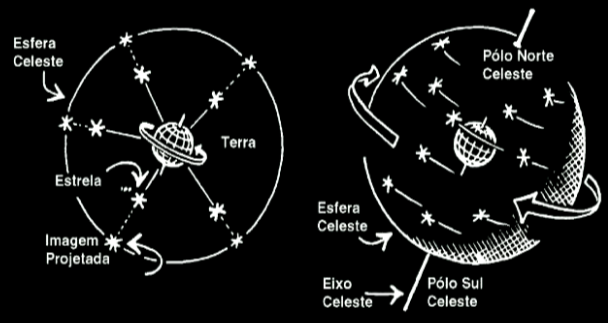
\includegraphics[width=7cm]{imagens/esfera_celeste.png}
    \caption{Exemplo de esfera celeste}
\end{figure}

\begin{itemize}
    \item \textbf{Zênite:} ponto mais alto na esfera celeste (direção vertical)
    \item \textbf{Nadir:} oposto ao Zênite 
    \item \textbf{Horizonte:} divisão entre a terra (plana localmente) e o céu  
    \item \textbf{Meridiano local:} de um polo ao outro passando pelo Zênite
\end{itemize}

Nos polos, conseguimos ver a tragetória dos astros na horizontal, no
Equador é perpendicular. Já entre os polos, os trajetos são inclinados na 
direção ao polo oposto

\begin{figure}[H]
    \centering
    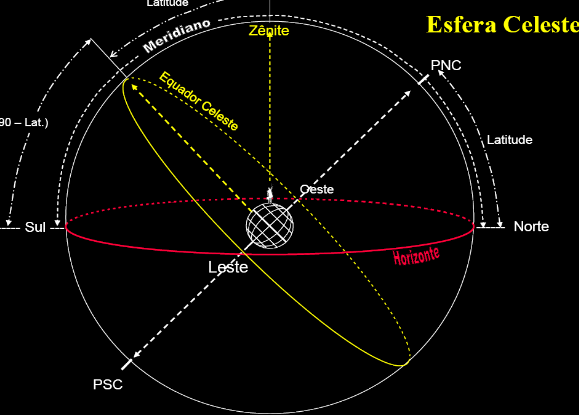
\includegraphics[width=7cm]{imagens/esfera_det.png}
    \caption{Detalhamento da esfera celeste}
\end{figure}

Sol nasce na direção leste, mas o local exato varia ao longo do ano 

\begin{figure}[H]
    \centering
    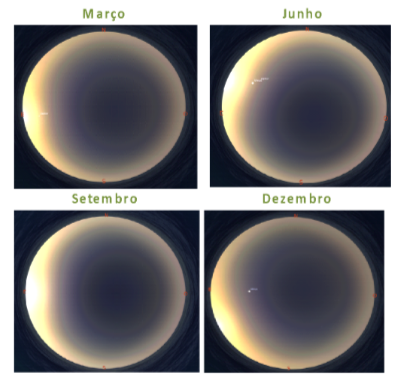
\includegraphics[width=7cm]{imagens/mov_sol.png}
    \caption{O sol se move para o norte ou sul dependendo da época do ano}
\end{figure}

\begin{figure}[H]
    \centering
    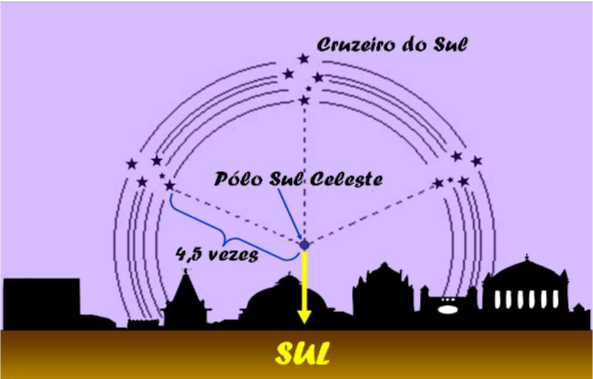
\includegraphics[width=7cm]{imagens/cruzeiro_sul.png}
    \caption{Cruzeiro do Sul: constelação circunpolar cujo eixo maior (ponra da cruz)
    aponta da direção do polo celeste sul}
\end{figure}



\begin{figure}[H]
    \centering
    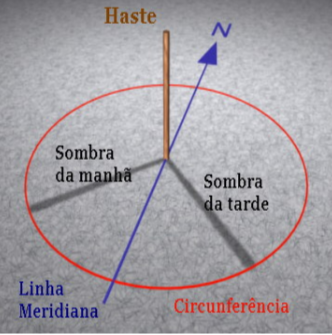
\includegraphics[width=7cm]{imagens/cardeais.png}
    \caption{Forma alternativa de verificar os pontos cardeais}
\end{figure}

Os gregos diferenciavam os astros em estelas fixas e errantes (ou planetas), que se 
moviam) $\leftarrow$ trajetória aparente eclíptica

\subsection{Modelo Geocêntrico}

Hiparco fez o primeiro catálogo estelar, com a posição do céu dos 
objetos (\textbf{coordenadas celestes}), além disso, dividiu estelas 
em magnitude (pelo brilho aparente)

Hiparco percebeu que a posição no céu do polo norte mudou em 150 anos
e a direção aparente da rotação do céu pareceu mudar também.

A direção do eixo da Terra realemnte muda lentamente (movimento de 
precessão)

Ptolomeu fez um modelo do sistema solar geocêntrico que pendurou 
por mais de 1000 anos


\begin{figure}[H]
    \centering
    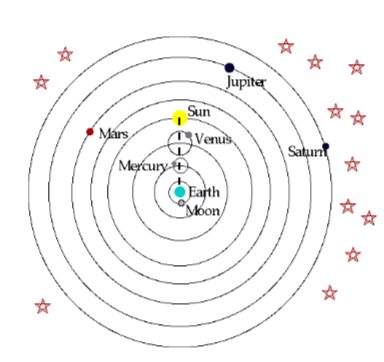
\includegraphics[width=7cm]{imagens/modelo_ptolom.png}
    \caption{Modelo do Sistema Solar de Ptolomeu}
\end{figure}

Dificuldade: explicar movimento "não esperado" dos planetas, que 
hoje sabemos ser resultante da combinação dos movimentos deles com o 
da Terra 

\begin{figure}[H]
    \centering
    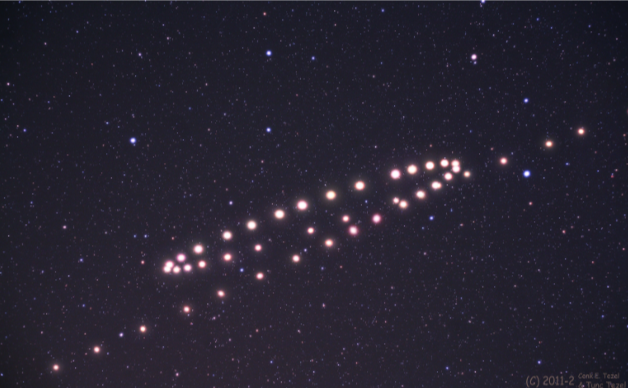
\includegraphics[width=7cm]{imagens/mov_marte.png}
    \caption{Movimento retrógrado de marte}
\end{figure}

O movimento retrógrado é tranquilo de explicar com o movimento da Terra
mas Ptolomeu partia do princípio que a Terra era estática e que o 
movimento dos astros era circular (gregos)

Ele propôs uma estrutura complexa de círculos movendo-se no interior
de outros círculos, introduzindo o conceito de \textbf{epiciclos} (movimento 
retrógrado), \textbf{deferente} e \textbf{equante} (variações de 
velocidade)

\subsection{Renascimento da Astronomia}

Com a expansão do Islamismo, a astronomia renasceu através da cultura
árabe  e judaica que preservavam ideias astronômica dos gregos 
antigos

Uma das ideias mais importantes 
do renascimento foi retirar a Terra do centro do Universo. Copérnico
concluiu que a Terra é um planeta que gira em torno do Sol (assim 
como os outros planetas). Somente a Lua circundava a Terra. 

\subsection{Modelo Heliocêntrico}

\begin{itemize}
    \item sol posicionado no centro
    \item Terra é um planeta que gira ao redor do sol
    \item ordem dos planetas desde o Sol: Mercúrio, Vênus, Terra, Marte, Júpiter e Saturno
    \item mais próximo o planeta estiver do Sol maior será sua velocidade orbital]
    \item Esse novo modelo explicava o movimento retrógrado !
\end{itemize}

\subsection{Observatório de Tycho Brahe}

Tycho detectou variações no movimento dos planetas daqueles 
previstos pelo modelo ptolomaico, mas tentava explicar com o 
geocentrismo.
Todo seu legado observacional foi herdado por  Kepler, logo após 
a sua morte.

\subsection{Galileu Galilei}

Descobriu que

\begin{itemize}
    \item existiam muitas estrelas fracas que só podiam ser vistas com 
    o telescópio
    \item conglomerados estelares
    \item Via Láctea é um “amontoado” de estrelas
    \item Quatro satélites de Júpiter e determinou seus períodos 
    (provando que nem tudo girava em torno da Terra)
    \item As fases de Vênus (não pode ser explicada por nenhum 
    modelo no qual Vênus circunda a Terra)
\end{itemize}

\subsection{Kepler}

Leis do movimento planetário descobertas por Kepler:

\begin{itemize}
    \item as órbitas de todos os planetas são elípticos
    \item linha que liga o planeta ao sol percorre áreas iguais em 
    tempo iguais
    \item Os quadrados dos períodos de translação dos planetas 
    são proporcionais aos cubos dos semi-eixos maiores de suas órbitas
\end{itemize}

\subsection{Newton}

Explicou a razão para os planetas seguirem as leias do movimento 
delineadas por Galileu, Tycho e Kepler

\begin{itemize}
    \item [I] Todo corpo continua em seu estado de repouso ou de 
    movimento uniforme em uma linha reta, a menos que seja forçado 
    a mudar aquele estado por forças aplicadas sobre ele (lei da inércia).
    \item [II] A mudança de movimento é proporcional à força motora 
    imprimida, e é produzida na direção de linha reta na qual aquela 
    força é imprimida. $F = m a$
    \item [III] A toda ação há sempre uma reação oposta e de igual 
    intensidade: ou as ações mútuas de dois corpos um sobre o outro 
    são sempre iguais e dirigidas em direções opostas. 
\end{itemize}

\subsection{Lei da Gravidade}

Então porque o movimento dos planetas é descrito por elipses ?

\textbf{Hipótese de Newton:} A gravidade não é uma força limitada 
somente ao nosso planeta. Ela é a força universal de atração entre 
todos os corpos – atração universal entre os corpos. 

$$F_G = \frac{GM_1M_2}{R^2}$$

Newton foi capaz de expressar matematicamente que as únicas órbitas 
permitidas para os planetas seriam seções cônicas, dentre as quais 
a elipse descrita pela lei de Kepler

\subsection{Movimento orbital e a massa}

Com a gravitação de NEwton deduzimos a 3ª Lei de Kepler:

$$\rho = D^3 \frac{4\pi^2}{GM_1M_2}$$

Aliás, Netuno foi descoberto ao observar uma irregularidade no
movimento previsto para Urano

\subsection{Movimento aparente}

\textbf{Eclíptica:} caminho aparente percorrido pelo Sol a cada 
ano, projetado na esfera celeste (Sol gradativamente muda sua 
posição na esfera celeste, movendo-se a cada dia 1° para leste 
em relação as outras estrelas da esfera celeste –  esse 
movimento completo leva o período de um ano)

Asterismos: São grupos de estrelas no céu que formam uma 
figura que seja facilmente identificável

\subsection{Medidas de Tempo}

As medidas do tempo e os calendários são baseados nos 
movimentos de rotação e translação da Terra e translação da Lua
Plano de referência é o Meridiano do observador !
(plano que passa pelo zênite local e pelos polos N e S geográficos 
e celestes.)

\section{Dia e Noite}

Movimento aparente de leste a oeste do sol se deve ao movimento de 
rotação de oeste a leste da terra em seu eixo.

Estações do ano estão relacionadas à inclinação do eixo da terra
em relação ao plano do sol, já que a incidência de raios de luz 
aumenta (ou diminui)

Dezembro: verão no hemisfério sul, no polo sul sol não se põe e 
Terra se encontra no periélio (ponto mais próximo do sol)



\end{document}